\chapter{Introduction}

\section{Background}

The self-organisation of cells into an apparent order appears across many different fields within developmental biology for example, the distribution of cells during the development process of an embryo, the growth of cancerous tissue \cite{morph}, vertebrate limb development \cite{miura1,glimm,miura2}, and pattern formation on animal coats (e.g spots on a jaguar \cite{painter}, feathers on birds \cite{bailleul}). Wolpert \cite{wolpert} presented the idea that, underpinning the development of shape and form (morphogenesis) is a cell's ability to differentiate according to its position in space and time. Furthermore, the concentration of certain chemicals (morphogens), or the concentration gradients of certain morphogens across a spatial domain of cells, affects the cell differentiation mechanism, and thus cells adopt a state relative to the concentration of a specific morphogen that they are exposed to.

In 1952 \cite{turing}, Alan Turing proposed that the morphogenesis process could be mathematically modelled as a purely chemical basis via the interaction of morphogens, whose evolutions are described by a system of coupled reaction-diffusion equations. It was proposed that a stable steady-state, robust to small perturbations in the spatially homogeneous setting, could become unstable and sensitive to small perturbations with the introduction of diffusion, leading to spatially inhomogeneous patterns. The diffusive term acts as a transportation mechanism for the reactants across a sufficiently large spatial domain. Turing's theory is therefore one of pre-patterning formation, where the morphogen concentration gradients, and thus the chemical reactions between the morphogens, determine cell fate decisions.

The mechanism allowing cells to adopt an appropriate state is known as differential gene expression, and depends crucially on the communication between cells, achieved through cellular signalling \cite{gaffmonk}. Typical reaction-diffusion systems assume a negligible timescale on which the cellular signalling and gene expression processes occur. The gene expression process is however extremely complex and proceeds through several stages \cite{gaffmonk}, namely gene transcription and gene translation. These sub-processes can take large amounts of time, and it has been experimentally shown that these time delays are typically on the order of minutes, but in some cases can be as large as a few hours \cite{gaffmonk,tennyson}. These time delays can therefore be on the same order of magnitude as the pattern formation process itself. For example, the basic body plan of a zebrafish is established in less than 24 hours \cite{gaffmonk,kimmel}. It is therefore important to consider these delays when studying pattern formation in Turing mechanisms.

Such time delays have been investigated in the context of Turing patterns, both numerically and analytically. The numerical results in \cite{gaffmonk}, which studied the ligand-internalisation (LI) variant of the Schnakenberg model \cite{schnakenberg}, showed that time taken until pattern formation occurs drastically increases as the gene expression time delay in the model is increased, and that small delays can cause a large increase in time-to-pattern. Numerical simulations on a growing domain also suggested that time delay can cause a failure in Turing pattern formation. Similar results have also been discussed in \cite{leegaffney,leegaffmonk}, for both the LI and reverse-ligand bonding (RLB) variants of the Schnakenberg model, where simulations have shown the disruption time delay can cause to pattern formation, as well as inducing temporal oscillations and increasing sensitivity of Turing instabilities to initial conditions.

Such time delays have been investigated in the context of Turing patterns \cite{gaffmonk,leegaffney,yigaffneyli,jiang,leegaffmonk,bratsun,william}, by incorporating fixed constant delays into typical reactiond-diffusion systems.  Numerical simulations on a growing domain also suggested that time delay can cause a failure in Turing pattern formation. Similar results have also been discussed in \cite{leegaffney,leegaffmonk}, for both the LI and reverse-ligand bonding (RLB) variants of the Schnakenberg model, where simulations have shown the disruption time delay can cause to pattern formation, as well as inducing temporal oscillations and increasing sensitivity of Turing instabilities to initial conditions.

A study in \cite{yigaffneyli} for the LI and RLB models, using linear analysis, has shown that increasing time delay can antagonise the the induction of Turing patterns. The work in \cite{jiang} showed a vast range of possible behaviours obtainable in the RLB model, including both spatial and temporal oscillations. It has therefore in general been found that these time delays can increase the time taken until pattern formation occurs, induce oscillations, or completely prevent pattern formation, and therefore pose a potential obstacle to applying Turing models to real systems. Interestingly, more recently it has been observed in \cite{fadai} that introducing time delay in only the activator term of the reaction-diffusion mechanism for the Gierer-Meinhardt model can act as a stabilising agent for pattern formation and increase the parameter space where one might expect to find Turing patterns, compared to a no-delay model.

On a cellular level however, the biological processes responsible for gene expression are inherently stochastic \cite{raj,elowitz,mcadams,paulsson}. Introducing merely a fixed-delay term into the kinetic equations is an oversimplification of the underlying biological process on a microscopic, and leads us to consider a distribution of time delays at the macroscopic level \cite{bratsun,krausenew}. In this report we are interested in whether implementing different forms of the delay, namely distributed delay, can alleviate some of the problems caused by the fixed delay case.

We will first outline some of the mathematical preliminaries used throughout this paper, including an outline of Turing pattern theory, and the numerical methods we use. Chapter 2 will be concerned with verifying and extending the numerical results in current literature concerned with the fixed delay model, as well as looking at the presented theory in more depth. We will specifically be concerned with evaluating the robustness of current results to varying initial and boundary conditions. We also aim to analytically show the relationship between a fixed time delay, and the time taken for pattern formation to occur. Finally, Chapter 3 will focus on the distributed delay model. We aim to produce novel linear analysis for the distributed delay case and numerically verify any observations we make.
\section{Model Introduction}
\subsection{Without Time Delay}
The mathematical model we will consider is the Schnakenberg model \cite{schnakenberg} - one of the simplest `toy' models that exhibit some of the key behaviours that we are interested in, and has also been studied extensively in the context of fixed time delays. The model describes the evolution and interaction between two reactants, $U$ and $V$. Only considering two reactants is a gross simplification of the underlying biological processes responsible for pattern formation, but it is still a non-trivial case than can admit Turing instabilities. In this report, we restrict our investigation to one spatial domain. The chemical reaction describing the Schnakenberg kinetics is given by \cite{baker}
\begin{equation}\label{chem}
A\xrightleftharpoons[c_{-1}]{c_1} U,\quad B\xrightarrow{c_2} V,\quad 2U+V\xrightarrow{c_3} 3U
\end{equation}
where the reaction rates $c_i$ are taken to be $1$. $A$ and $B$ are substances whose evolution is non considered, and we assume a constant supply. We use $u$, $v$, $a$, and $b$ to denote the concentrations of substances $U$, $V$, $A$ and $B$ respectively. Letting the reactants diffuse, and applying the law of mass action yields the reaction-diffusion system
\begin{equation}\label{system}
    \begin{split}
    \frac{\partial u}{\partial t}&=\frac{\epsilon^2}{L^2}\frac{\partial^2 u}{\partial x^2}+a-u+u^2v,\\
    \frac{\partial v}{\partial t}&=\frac{1}{\L^2}\frac{\partial^2 v}{\partial x^2}+b-u^2v \quad\quad\quad x\in\Omega,
    \end{split}
\end{equation}
where $\Omega$ is the non-dimensionalised spatial domain, which we consider here as $\Omega=[0,1]$ and where $a$ and $b$ are fixed parameters. Since we are interested in the pattern formation arising from the self-organisation of cells, we implement no flux (homogeneous Neumann) boundary conditions on the boundary of the spatial domain $\partial\Omega$, namely $\frac{\partial u}{\partial x}=\frac{\partial v}{\partial x}=0$ at $x=0, 1$. As typical when studying Turing patterns, initial conditions will be chosen as a small random perturbation from the spatially homogeneous steady state. The parameter $\epsilon^2$ can be thought of as the ratio of diffusion coefficients between the activator $u$ and inhibitor $v$, and $L^2$ a scaling of the domain length on which the problem is being solved. The choice of diffusion coefficients used in this report is motivated from those considered in \cite{gaffmonk}, where $\epsilon^2=0.001$ and $L=\sqrt{0.05}$. In this report, unless otherwise states, we take $\epsilon^2=0.001$ and use a larger domain size $L=30\sqrt{0.05}$.

\subsection{With Fixed Time Delay}

The form of the model we consider with fixed time delay is the ligand-internalisation (LI) variant of the standard Schnakenberg model. The LI model assumes that a reaction at the cell surface is followed by internalisation of a morphogen before the gene expression process can continue and morphogen production can occur \cite{leegaffney,yigaffneyli}. The time-delayed terms in the LI model only appear in the activator's dynamics. This is based on the assumption that the gene expression process, and thus the source of the time delay, is responsible for autocatalysis of the activator in the reaction-diffusion mechanism \cite{gaffmonk}. Applying the delay to the kinetics in the cubic nonlinearity term \cite{baker} in \eqref{chem} yields the reaction described by
\begin{equation}\label{chem2}
A\xrightleftharpoons[c_{-1}]{c_1} U,\quad B\xrightarrow{c_2} V,\quad 2U+V\xrightarrow{c_3} W\quad W\xrightarrow{\text{\footnotesize delay } \tau}3U,
\end{equation}
where the reaction rates $c_i=1$. The reaction describes an internalisation of two particles of $U$, and one particle of $V$, which are removed from the reaction, represented by substance $W$. However, three particles of $U$ are obtained from a reaction at a time $\tau$ in the past. The reaction-diffusion system describing the LI model is thus written as \cite{leegaffney}
\begin{equation}\label{fixed}
  \begin{split}
  \frac{\partial u}{\partial t}&=\frac{\epsilon^2}{L^2}\frac{\partial^2u}{\partial x^2}+a-u-2u^2v+3\hat{u}^2\hat{v}\\
  \frac{\partial v}{\partial t}&=\frac{1}{L^2}\frac{\partial^2v}{\partial x^2}+b-u^2v,
\end{split}
\end{equation}
where $u=u(x,t)$, $v=v(x,t)$ and $\hat{u}$, $\hat{v}$ are evaluated at some delay $\tau$, so that $\hat{u}=u(x,t-\tau)$ and $\hat{v}=v(x,t-\tau)$.

\subsection{With Distributed Time Delay}

The stochastic nature of gene expression delays leads us to consider a mean-field approach to modelling the time delay \cite{bratsun,krausenew}. As done in \cite{william}, by assuming each individual mechanism within the gene expression process acts independently and identically, we use the central limit theorem to model the delay as a Gaussian distribution with some mean $\tau$ and standard deviation $\sigma$. We begin by using a symmetric truncated Guassian distribution, with integration limits $a=\tau-n\sigma$ and $b=\tau+n\sigma$ for some $n\in\mathbb{N}$, such that $a=\tau-n\sigma>0$ to maintain positive time delays. We can thus write the LI model with distributed time delay as

\begin{equation}\label{distmodel}
  \begin{split}
    \frac{\partial u}{\partial t}&=\frac{\epsilon^2}{L^2}\frac{\partial^2u}{\partial x^2}+a-u-2u^2v+3\int_{a}^{b}k(s,\tau,\sigma)\hat{u}^2\hat{v} \ \text{ds},\\
    \frac{\partial v}{\partial t}&=\frac{1}{L^2}\frac{\partial^2v}{\partial x^2}+b-u^2v,
\end{split}
\end{equation}
where $\hat{u}=u(x,t-s)$ and $\hat{v}=v(x,t-s)$, with $s$ the integration variable ranging over the delays. The function $k(s,\tau,\sigma)$ is the truncated Gaussian pdf given by \cite{wikitrunc}
\begin{equation}
  k(s)=\frac{\Phi_c}{\sqrt{2\pi}\sigma}\exp\left(\frac{-1}{2}\left(\frac{s-\tau}{\sigma}\right)^2\right).
\end{equation}
We use $\Phi_c$ to denote the truncation scaling constant. This constant ensures $k(s,\tau,\sigma)$ integrates to $1$ over the given integration domain $[a, b]$, and is computed as
\begin{equation}
\Phi_c=\frac{1}{\phi\left(\frac{b-\tau}{\sigma}\right)-\phi\left(\frac{a-\tau}{\sigma}\right)},
\end{equation}
with the function $\phi$ described by
\begin{equation}
\phi(x)=\frac{1}{2}\left(1+\text{erf}\left(\frac{x}{\sqrt{2}}\right)\right).
\end{equation}
In order to numerically study the distributed delay model, we will use the composite Simpson's rule to evaluate the integral term. This will be studied in more detail in section \ref{section:quad}.

\section{Mathematical Preliminaries}
\subsection{Turing Pattern Formation Without Delay}
Here we give a brief overview of the mathematical theory underpinning Turing pattern formation, closely following the description in \cite{murray}. For further details, the reader should consult \cite{murray,beentjes}. Turing patterns occur when the spatially homogeneous stable steady-state becomes unstable in the presence of diffusion. We therefore first consider the spatially homogeneous model, and explore conditions necessary for the steady-state to be stable. In the case of the Schnakenberg model, the single steady-state, $(u_\star, v_\star)$, occurs at $(u_\star, v_\star)=\left(a+b, \frac{b}{(a+b)^2}\right)$. Since $a,b>0$, we have $u_\star,v_\star>0$. Following the methodology in \cite{murray}, we perform linear stability analysis. Taking a small perturbation from the steady-state, so that $\hat{u}=u-u_\star$, $\hat{v}=v-v_\star$ for $|\hat{u}|, |\hat{v}|<<1$, we consider the evolution of the perturbation. Denoting $\hat{\textbf{u}}$ as the vector of perturbations, $\hat{\textbf{u}}=\begin{bmatrix}\hat{u} \\ \hat{v}\end{bmatrix}$, the linearised system of \eqref{system} is given as
\begin{equation}\label{linsys}
\frac{\text{d}\hat{\textbf{u}}}{\text{dt}}=\textbf{J}_{(u_\star,v_\star)}\hat{\textbf{u}},
\end{equation}
where $\textbf{J}_{(u_\star,v_\star)}$ is the Jacobian matrix of the kinetic equations evaluated at the steady-state. Namely,
$$
\textbf{J}_{(u_\star,v_\star)}=\begin{pmatrix}f_u&f_v\\g_u&g_v\end{pmatrix}\Bigg|_{(u_\star,v_\star)}.
$$
The notation $f_u$ is used to denote the partial derivatve of $f$ with respect to $u$. Solutions of \eqref{linsys} are of the form
$$
\hat{\textbf{u}}\propto e^{\lambda t},
$$
for eigenvalues $\lambda$ of $J_{(u_\star,v_\star)}$. The steady-state is asymptotically stable if the perturbation decays.
Denoting $\text{spec}(\textbf{M})$ as the set of eigenvalues of some matrix $\textbf{M}$, asymptotic stability occurs when $\Re(\lambda)<0 \ \text{for all }\lambda\in \text{spec}(\textbf{J}_{(u_\star,v_\star)})$. However, if there exists $\lambda\in \text{spec}(\textbf{J}_{(u_\star,v_\star)})\text{such that } \Re(\lambda)>0$,
then the pertubation will grow with time and the steady-state in unstable. The sum and product of the eigenvalues of $\textbf{J}_{(u_\star,v_\star)}$
are given by $\text{Tr}(\textbf{J}_{(u_\star,v_\star)})$ and $\text{det}(\textbf{J}_{(u_\star,v_\star)})$ respectively. The required conditions for stability are therefore
\begin{equation}\label{cond1}
    \begin{split}
\text{Tr}(\textbf{J}_{(u_\star,v_\star)})<0 &\implies (f_u+g_v)\big|_{(u_\star,v_\star)}<0, \\
\text{det}(\textbf{J}_{(u_\star,v_\star)})>0 &\implies (f_ug_v-f_vg_u)\big|_{(u_\star,v_\star)}>0,
\end{split}
\end{equation}
We now consider the full diffusive model and look for necessary conditions such that the previously stable steady-state is driven to instability. The linearised system is given by
\begin{equation}\label{linsys2}
    \frac{\partial \hat{\textbf{u}}}{\partial t}=\left[\textbf{D}\nabla^2+\textbf{J}_{(u_\star,v_\star)} \right]\hat{\textbf{u}},
\end{equation}
where $\textbf{D}=\begin{pmatrix}\frac{\epsilon^2}{L^2}&0\\0&\frac{1}{L^2}\end{pmatrix}$ is the matrix containing the diffusion coefficients of reactants.
The solution to the spatially dependent eigenvalue problem can be written as a linear combination of the eigenfunctions $w_k$ that satisfy the problem
\begin{equation}\label{eigprob}
\nabla^2w_k=-k^2w_k,\quad \quad \frac{\partial w_k}{\partial \textbf{n}}=0\text{ for } \textbf{x}\in\partial\Omega.
\end{equation}
Considering only a regular 1D domain $\Omega=[0,1]$ with no flux boundary conditions, the eigenfunctions will be of the form $w_k=\cos(k\pi x)$, $x\in[0,1]$. $\partial\Omega$ denotes the boundary of the domain, and $\textbf{n}$ denotes the outward-facing normal.
We thus look for solutions to \eqref{linsys2} of the form
\begin{equation}\label{perturbgrow}
    \hat{\textbf{u}}=\sum_k \textbf{c}_ke^{\lambda_k t}w_k(x),
\end{equation}
where the constants $\textbf{c}_k$ are determined by using a Fourier expansion of the initial conditions in terms of the eigenfunctions $w_k$. $\lambda_k$ is the eigenvalue which determines the rate of temporal growth for each mode $k$, and thus determines whether a particular mode of pattern will be unstable and grow. Substituting this form \eqref{perturbgrow} into \eqref{linsys2}, along with using \eqref{eigprob} and simplifying, we obtain, for each $k$
$$
\lambda_k w_k=\textbf{J}w_k-\textbf{D}k^2w_k \implies (\lambda_k \textbf{I}-\textbf{J}+k^2\textbf{D})w_k=\textbf{0},
$$
with $\textbf{I}$ the identity matrix. Looking for non-trivial solutions for $w_k$, we set solve for roots of the characteristic polynomial, namely $\text{det}(\lambda_k \textbf{I}-\textbf{J}+k^2\textbf{D})=0$, which yields a quadratic equation for eigenvalues $\lambda_k(k)$ as a function of $k$. Finding roots of this quadratic such that $\Re(\lambda_k(k))>0$ for some $k\neq0$, we can conclude two necessary conditions for the instability of the steady-state in the presence of diffusion, namely
\begin{equation}\label{cond2}
    \begin{split}
    \left(\frac{1}{\epsilon^2}f_u+g_v\right)\bigg|_{(u_\star,v_\star)}>0&\\
    \left(\left(\frac{1}{\epsilon^2}f_u+g_v\right)^2-\frac{4}{\epsilon^2}(f_ug_v-f_vg_u)\right)\bigg|_{(u_\star,v_\star)}>0.
\end{split}
\end{equation}
We therefore have four necessary conditions in terms of $(a,b,\epsilon^2)$ for Turing patterns to occur. These conditions are only necessary, and not sufficient, as conditions \eqref{cond2} assume $k$ to be a continuous variable, rather than discrete, and this is only strictly valid in the limit $L\to\infty$. Using the first two conditions in \eqref{cond1}, a bifurcation diagram in the $(a,b)$ parameter space can be plotted showing the regions corresponding to a stable or unstable steady state. This can be seen in figure \ref{fig:bifsh}. Using the additional conditions in \eqref{cond2} and the fixed value $\epsilon^2=0.001$, the parameter region in the $(a,b)$ parameter space in which Turing patterns can occur can also be plotted. This `Turing space' can be seen in figure \ref{fig:turingspace}.

\begin{figure}[H]
    \centering
    \begin{subfigure}[b]{0.45\textwidth}
        \centering
        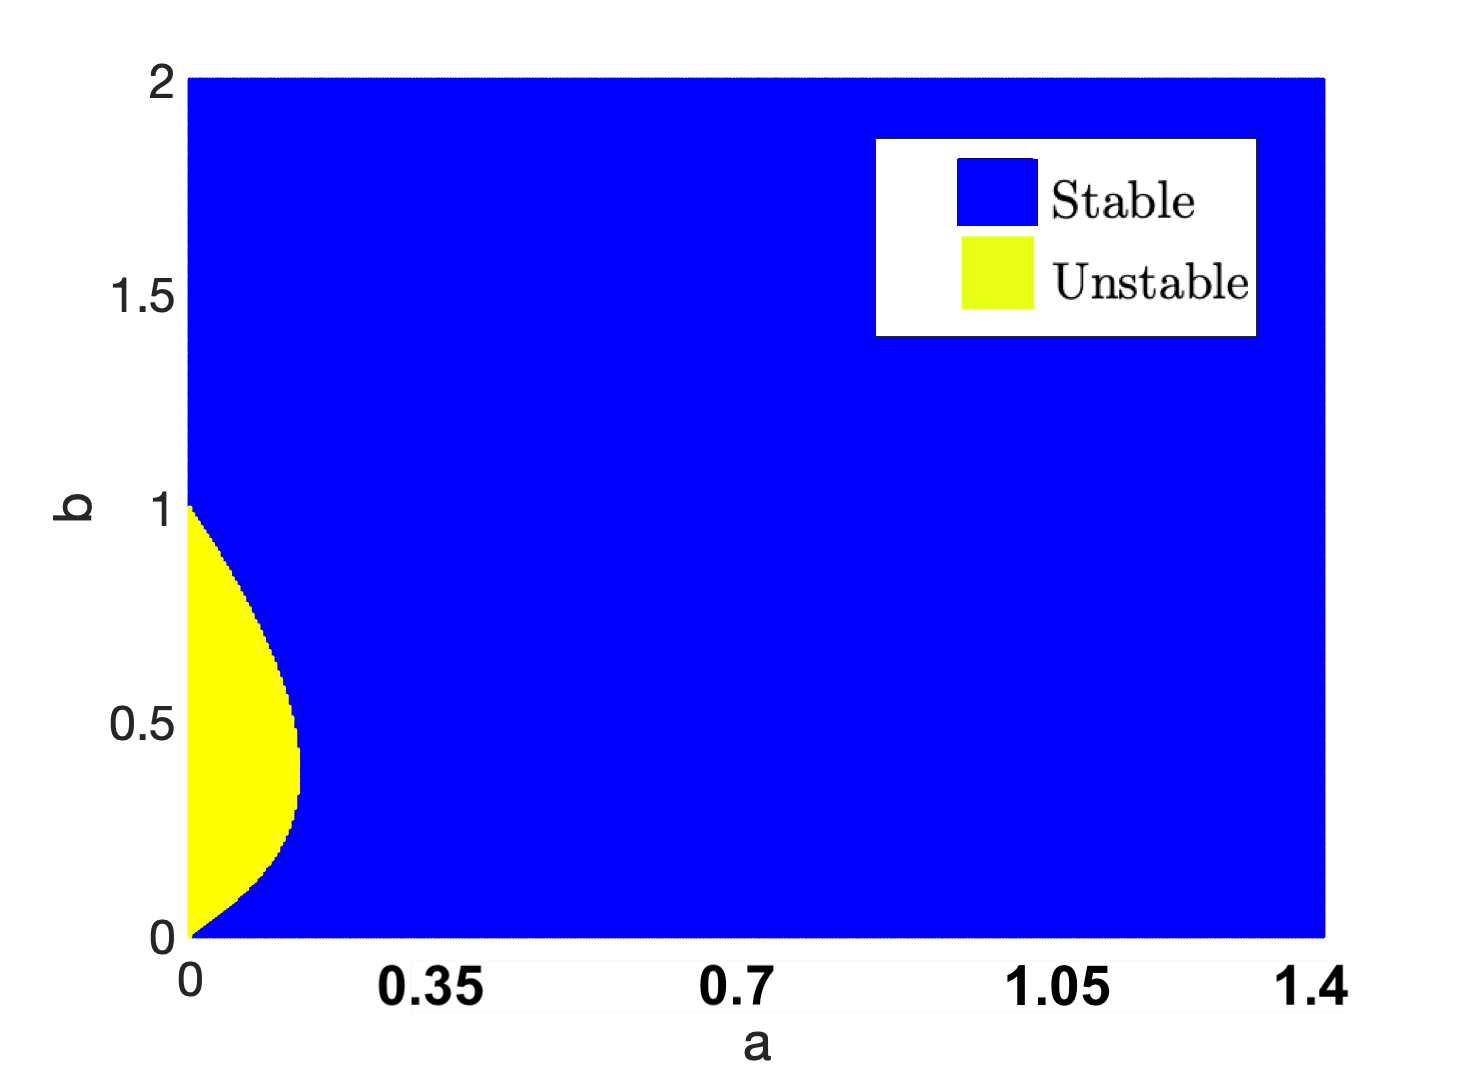
\includegraphics[width=8cm,height = 6cm]{bifsh.png}
        \caption{Bifurcation diagram for spatially homogeneous model, no delay.}
        \label{fig:bifsh}
    \end{subfigure}
    \hfill
    \begin{subfigure}[b]{0.45\textwidth}
        \centering
        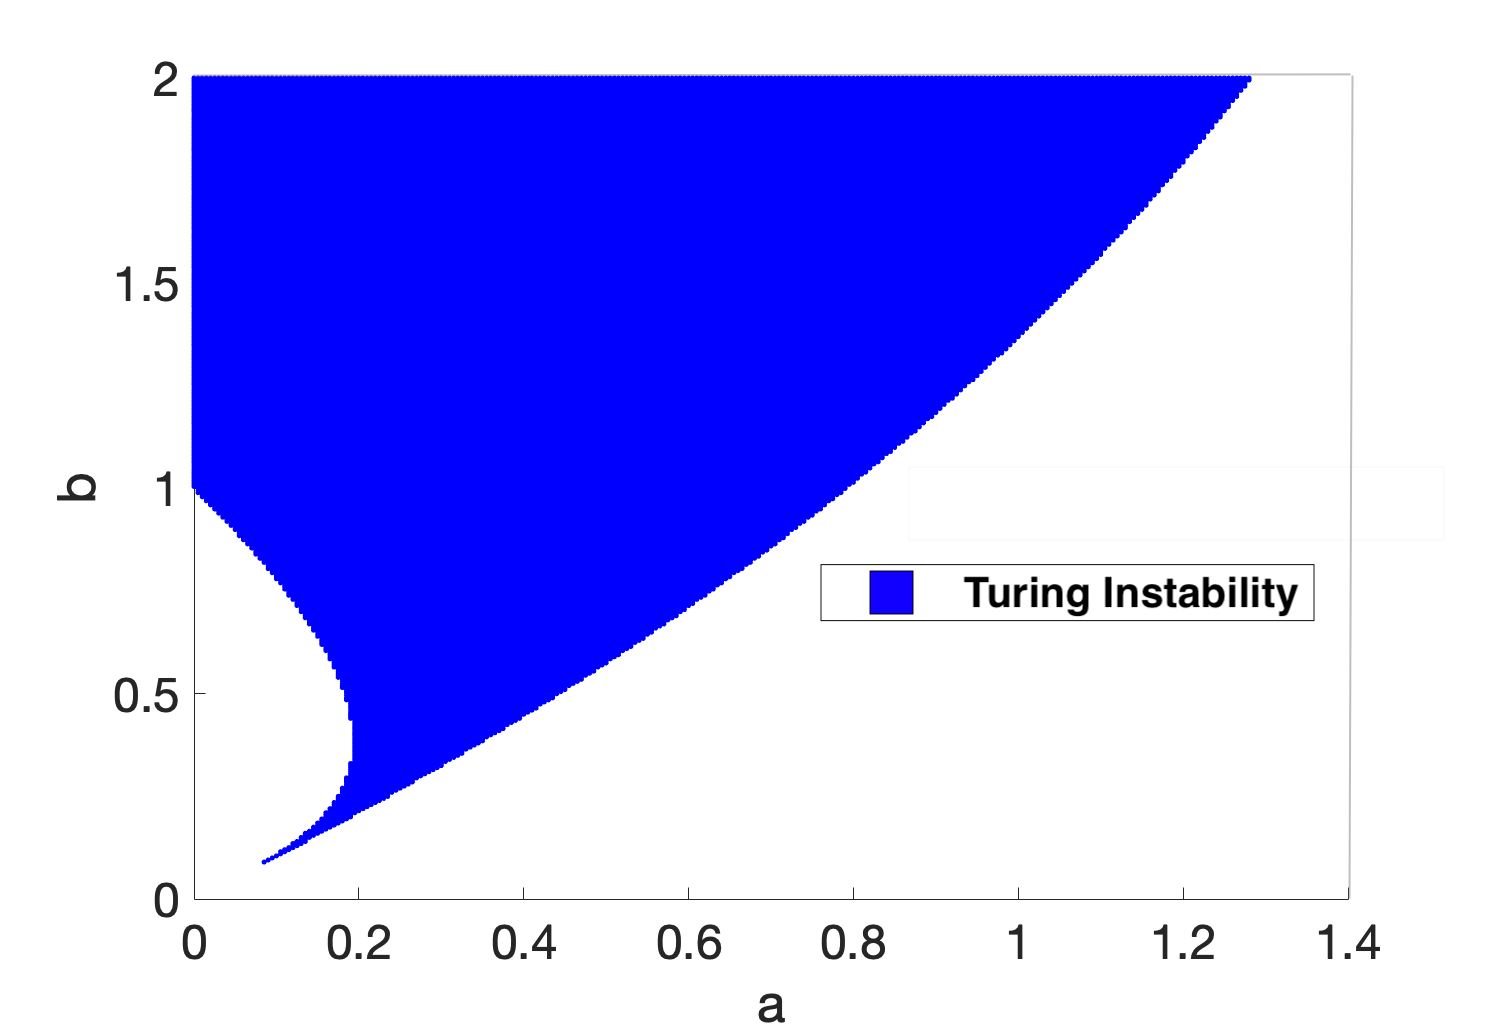
\includegraphics[width=8cm,height = 6cm]{turingspace.png}
        \caption{Turing space, no delay. $\epsilon^2=0.001$.}
        \label{fig:turingspace}
    \end{subfigure}
    \caption{Conditions \eqref{cond1} and \eqref{cond2} used to plot bifurcation diagram and Turing space for parameters $(a,b)\in[0,1.4]\times[0,2]$.}
    \label{fig:dispfixed}
\end{figure}

\subsection{Numerical Implementation}\label{section:numimp}
In order to numerically resolve the spatial derivatives $\frac{\partial^2 u}{\partial x^2}$, $\frac{\partial^2 v}{\partial x^2}$ and implement the relevant boundary conditions, a finite-difference scheme is used. Throughout the report we use $m=500$ equally spaced spatial discretisation points on the domain $x\in\Omega=[0,1]$. Further details on the derivation and implementation of the finite difference scheme with both homogeneous Dirichlet and Neumann conditions can be found in appendix \ref{section:appA}.
\\
Reaction-diffusion systems can be numerically stiff to solve \cite{stiff1, william}, and thus to solve these systems with time delay, we require stiff numerical solvers suitable for delay differential equations (DDEs). The inherent stiffness of the problem makes standard DDE solvers in MATLAB such as \emph{dde23} and \emph{ddesd} unsuitable, and past work has been restricted in the progress made through numerical simulations \cite{william} due to the computationally expensive task of solving reaction-diffusion systems with non-stiff solvers. Standard stiff solvers in MATLAB, such as \emph{ode23s} and \emph{ode15s} do not support time delay. We therefore use the Julia language to numerically solve these systems. Julia has an extensive differential equations solver suite \cite{rodas}, and has the capability to apply the method of steps \cite{methsteps} to a stiff solver, allowing the incorporation of fixed time delays. Throughout the report we use absolute and relative solver tolerances of $10^{-6}$, with a maximum timestep set as $0.1$. For these tolerances, the default stiff solver implemented by Julia is \emph{Rodas5}, a 5-th order A-stable solver, from the family of Rosenbrock methods \cite{rodas}. An interested reader can find more details on Rosenbrock methods in \cite{rosenbrock}.
